\section{Dämmstoffe}
\BlueSectionSlide


\begin{frame}{Besprechung des Quiz}

\end{frame}


\begin{frame}{Einheit der Wärmeleitfähigkeit}
	\begin{Definition_BS}{Wärmeleitfähigkeit}
		Die Wärmeleitfähigkeit $\lambda$ ist eine Materialkonstante, die angibt, wie gut ein Material Wärme leitet. Sie wird in der Einheit \si{\watt\per\meter\per\kelvin} angegeben.
	\end{Definition_BS}
	\pause
	\begin{Beispiel}{Wärmeleitfähigkeit von einigen Materialien}
		\begin{itemize}
			\item[\textbullet] \textbf{Holz:} $\lambda = \SI{0.1}{\watt\per\meter\per\kelvin}$
			\item[\textbullet] \textbf{Beton:} $\lambda = \SI{1.5}{\watt\per\meter\per\kelvin}$
			\item[\textbullet] \textbf{Luft:} $\lambda = \SI{0.025}{\watt\per\meter\per\kelvin}$
		\end{itemize}
	\end{Beispiel}
\end{frame}

\begin{frame}{Steinwolle besteht aus:}
    \begin{Fragenblock}
        Steinwolle besteht aus:
        
        \begin{itemize}
            \item[\faSquare] künstlichen Mineralfasern
            \item[\faSquare] natürlichen Mineralfasern
        \end{itemize}
    \end{Fragenblock}
\end{frame}

\begin{frame}{Steinwolle besteht aus:}
    \begin{Fragenblock}
        Steinwolle besteht aus:
        
        \begin{itemize}
			\item[\textcolor{green!70!black}{\faCheckSquare}] künstlichen Mineralfasern
			\item[\faSquare] natürlichen Mineralfasern
        \end{itemize}
    \end{Fragenblock}
\end{frame}

\begin{frame}{Steinwolle ist resistent gegen Fäulnis?}
    \begin{Fragenblock}
        Steinwolle ist resistent gegen Fäulnis?
        
        \begin{itemize}
            \item[\faSquare] Richtig
            \item[\faSquare] Falsch
        \end{itemize}
    \end{Fragenblock}
\end{frame}

\begin{frame}{Steinwolle ist resistent gegen Fäulnis?}
    \begin{Fragenblock}
        Steinwolle ist resistent gegen Fäulnis?
        
        \begin{itemize}
			\item[\textcolor{green!70!black}{\faCheckSquare}] Richtig
			\item[\faSquare] Falsch
        \end{itemize}
    \end{Fragenblock}
\end{frame}


\begin{frame}{Glaswolle vs. Steinwolle}

	\begin{block}{Steinwolle}
		\ldots ist für gewöhnlich gelbgrün bis graugrün.
	\end{block}
	\pause
	\begin{block}{Glaswolle}
		\ldots zeigt eine gelbe, weisse oder braune Farbgebung auf.
	\end{block}
\end{frame}

\begin{frame}{Weisses Granulat}

    \begin{figure}[H]
        \centering
        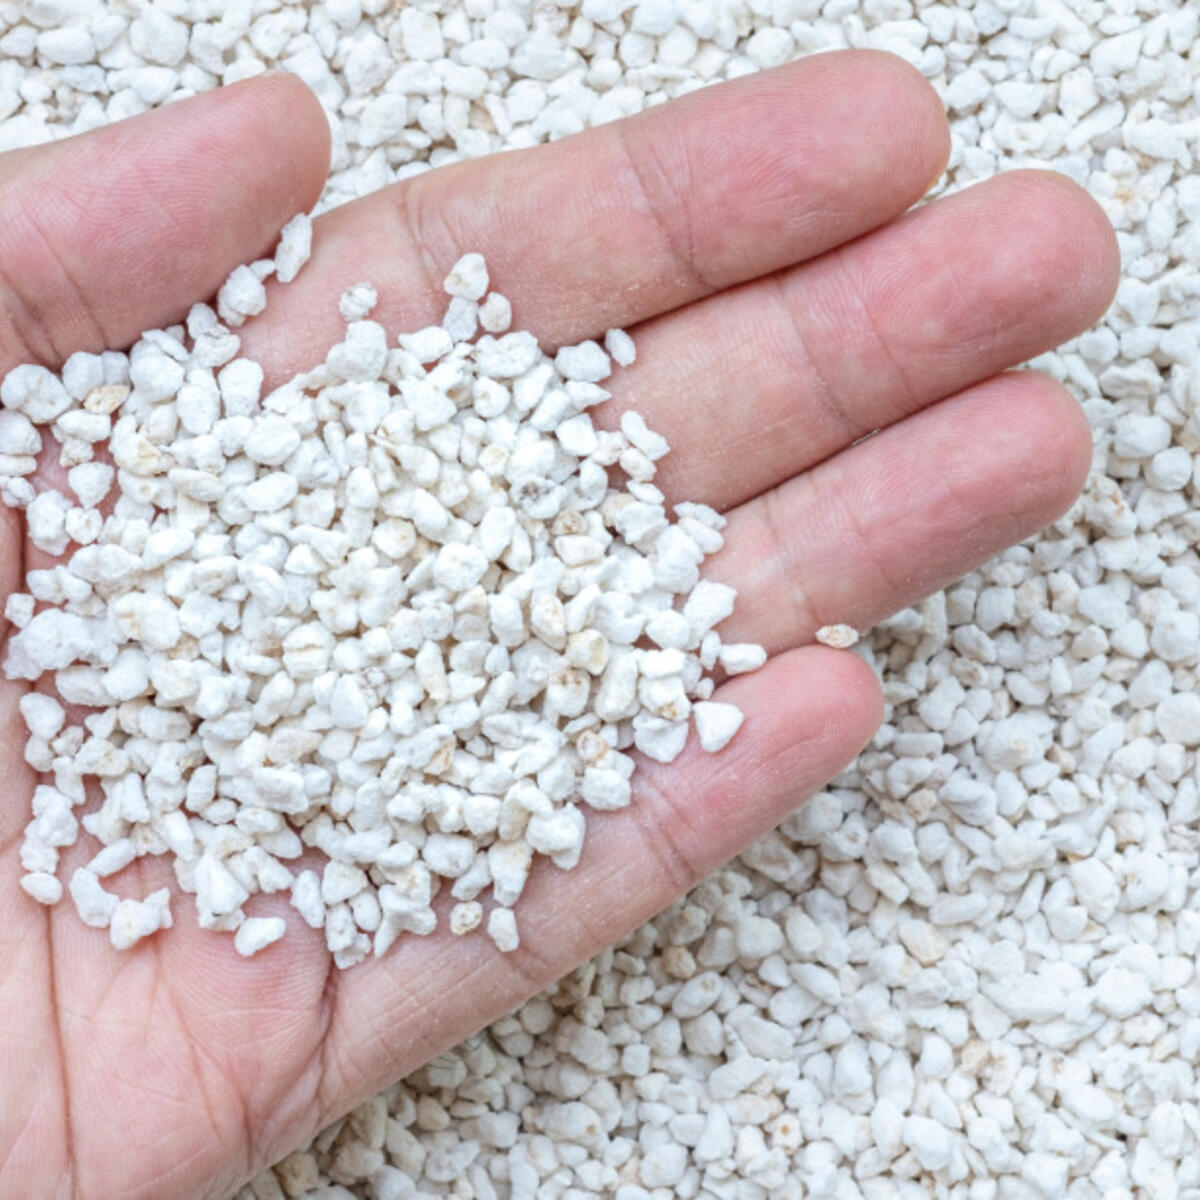
\includegraphics[height=0.7\textheight]{/Users/patricpf/Documents/repos/Bauschule-Baustoffe/Unterlagen/12_WDS/Bilder/Perlit.jpg}
        \caption{Perlit. (Styropor ist ein Markenname für Polystyrol und bereits eine Platte.)}
    \end{figure}


\end{frame}

\frageMitZweiFolien{Eigenschaften von Schurwolle}{Dämmstoffe aus Schurwolle haben eine hohe Speicherkapazität von Luftfeuchtigkeit.}{richtig}

\frageMitZweiFolien{Eigenschaften von Holzwollplatten}{Holzwollplatten sind bekannt als sehr guter Dämmstoff.}{falsch}

\frageMitZweiFolien{Zellulosefasern}{Isofloc ist ein bekanntes Produkt für Dämmstoffe aus Zellulosefasern.}{richtig}

\frageMitZweiFolien{Bindemitteln von Holzwollplatten}{Holzwollplatten werden i.d.R. mit Zement oder Gips gebunden.
}{richtig}

\frageMitZweiFolien{Eigenschaften von Holzfasterplatten}{Holzfaserplatten haben i.d.R. eine gute Wärme und ein gute Schalldämmung.
}{richtig}

\frageMitZweiFolien{Expansion von PS-Gries}{Das Polystyrolgries wird auf das ca. 20-fache seines Ausgangsvolumen aufgebläht.
}{falsch}

\frageMitZweiFolien{Produktname: Styrofoam}{Styrofoam ist ein XPS-Produkt.
}{richtig}


\begin{frame}{$\lambda$-Wert- Berechnungen}

	Bitte nochmals vor der Prüfung individuell anschauen.

\end{frame}